\documentclass[12pt, letterpaper]{article}
%\documentclass[12pt, letterpaper]{amsart}

%%%%%%%%%%%% LANGUAGE & ENCODING %%%%%%%%%%%%%%%%%
\usepackage[english]{babel}
\usepackage[utf8]{inputenc}%%%% to process umlauts and accents directly
%\usepackage{indentfirst}
%\usepackage{ucs}

%%%%%%%%%%% PACKAGES %%%%%%%%%%%%%%%%%%%%%%%%%%%%%
% For Hyperlinks
\usepackage[colorlinks,linkcolor=cyan,citecolor=magenta]{hyperref}

% Common math packages
\usepackage{amsthm, amsmath, amsfonts, amssymb, esint, mathrsfs, mathtools}
\usepackage{tensor} % To handle multi-index notation
\usepackage[capitalize,nameinlink]{cleveref} % Nice references
\crefname{equation}{}{} % Removes Eq. from equation references
\numberwithin{equation}{section} % Number equations within each section separately

% Extra symbols
\usepackage{stmaryrd} % contains \owedge  for Kulkarni-Nomizu product and some other special characters
\usepackage{commath} % contains \norm \abs

% Some useful packages
\usepackage{verbatim} %%% enables \begin{comment}    \end{comment}
\usepackage{enumerate} % allows different types of indices
\usepackage{float} % Handling figures

%%%%%%%%%%% MARGINS %%%%%%%%%%%%%%%%%%%%%%%%%%%%%%%%
% Margins
\usepackage[top=1in, bottom=1in, left=1in, right=1in]{geometry}

%%%%%%%%%%% CUSTOM NOTATION  %%%%%%%%%%%%%%%%%%%%%%
\newcommand{\N}{\mathbb{N}}
\newcommand{\Z}{\mathbb{Z}}
\newcommand{\Q}{\mathbb{Q}}
\newcommand{\R}{\mathbb{R}}
\newcommand{\C}{\mathbb{C}}
\newcommand{\K}{\mathbb{K}}

\newcommand{\f}{\mathfrak}
\newcommand{\ul}{\underline}
\newcommand{\mb}{\mathbb}
\newcommand{\mr}{\mathrm}
\newcommand{\mf}{\mathbf}
\newcommand{\mc}{\mathcal}
\newcommand{\e}{\emph}
\newcommand{\vp}{\varphi}
\newcommand{\ve}{\varepsilon}

\newcommand{\vol}{\operatorname{Vol}}
\newcommand{\diam}{\operatorname{diam}}
\newcommand{\dist}{\operatorname{dist}}
\newcommand{\dv}{\operatorname{div}}
\newcommand{\tr}{\operatorname{tr}}

\newcommand{\dd}{\; \mathrm{d}} %%%% d for integration dx
\newcommand{\wt}{\widetilde}
\newcommand{\ol}{\overline}

%%%%%%%%%%% THEOREMS %%%%%%%%%%%%%%%%%%%%%%%%
\newtheorem{theorem}{Theorem}[section]
\newtheorem{lemma}[theorem]{Lemma}
\newtheorem{proposition}[theorem]{Proposition}
\newtheorem{conjecture}[theorem]{Conjecture}
\newtheorem{corollary}[theorem]{Corollary}
\newtheorem{claim}[theorem]{Claim}
\newtheorem{problem}[theorem]{Problem}
\newtheorem{remark}[theorem]{Remark}

\theoremstyle{definition}
\newtheorem{definition}[theorem]{Definition}

\theoremstyle{remark}
\newtheorem{example}[theorem]{Example}


%%%%%%%%%%% TITLE %%%%%%%%%%%%%%%%%%%
%\title[CIS625: Computational Learning Theory]{Computational Learning Theory Lecture Notes}
%\author[Notes by Martin Citoler-Saumell]{Martin Citoler-Saumell}
%\date{Spring 2017}
%\address{University of Pennsylvania\\ Philadelphia, PA 19104}
%\email{\href{mailto:martinci@math.upenn.edu}{martinci@math.upenn.edu}}

\title{Computational Learning Theory Lecture Notes}
\author{Martin Citoler-Saumell}
\date{CIS625 Spring 2017}

%%%%%%%%%%% DOCUMENT BEGINS %%%%%%%%%%%%
\begin{document}
%------------------------------------------------------------
%          LECTURE 7
%------------------------------------------------------------
\section{Lecture 7: 2017.03.13}
\subsection*{Outline}
\begin{itemize}
\item SQ model: review  and lower bounds
\item PAC learning and cryptography
\item Boosting Part I
\end{itemize}

\subsection{Query complexity in SQ}
We saw that any PAC-learnable model can be framed in the SQ model by simulating the queries with enough draws from the distribution i.e calls to $EX(c, D)$. Intuitively,  the query complexity of the obtained model should not violate the lower bounds from previous lectures on the VCD.

\begin{claim}
Assume $VCD(\mc C)=d$, then at least $\Omega\left(\frac d{\log d}\right)$ queries with $\tau = O(\ve)$ are required in the SQ model.
\end{claim}
\begin{proof}[Sketch]
Let $\lbrace x_1,\ldots,x_d\rbrace$ be shattered by $\mc C$. Let $D$ such that $x_1$ has weight $1-3\ve$ and the rest have uniform weight $\frac{3d}{d-1}$. Consider the query $\chi = 1 \iff x=x_1\;\&\; y=0$, this allows the algorithm to learn the label of $x_1$. Now let $b_i = c(x_i)$, we must learn the labels of the majority of these labels. Specifying some other labels $c_i$, we can make statistical queries like $\mb P_i[b_i=c_i]$. For example, ``what is the proportion of 1's among $b_i$'s?''. This statistical query can be thought of as the inner product of this unknown $\vec b$ and any $\vec c$ that we want. Therefore, the learning problem reduces to a linear algebra problem.
\end{proof}

Recall the following remark from last time.
\begin{claim}
``Almost'' every PAC-learning algorithm has an SQ-algorithm.
\end{claim}

We can actually find counterexamples to the claim, hence the ``almost'' in the statement.
\subsubsection{PAC-learnable but not SQ-learnable}
Let $X=\lbrace 0,1 \rbrace$ and consider the parity functions over $X$. Namely, for any subset $S\subset \lbrace 1,\ldots, n\rbrace$ we can define
\begin{align}
f_S(\vec x) = \sum_ix_i \mod 2 \in \lbrace 0, 1\rbrace,
\end{align}
and the associated pairs $\langle \vec x, f_S(\vec x)\rangle$. They count the parity of the 1 bits in the set $S$. Note that $\abs{\mc C} = 2^n$. It turns out that this is PAC-learnable because examples correspond to linear equations but you can't can get the same information statistically. We have the info-theoretical result.
\begin{theorem}
Parity functions satisfy the following:
\begin{enumerate}[i)]
\item PAC-learnable (poly time \& samples)
\item Provably require exponential in n queries in SQ.
\end{enumerate}
\end{theorem}
\begin{proof}[Intuition]
Let $D$ be uniform over $X$.
\begin{figure}[H]
\centering
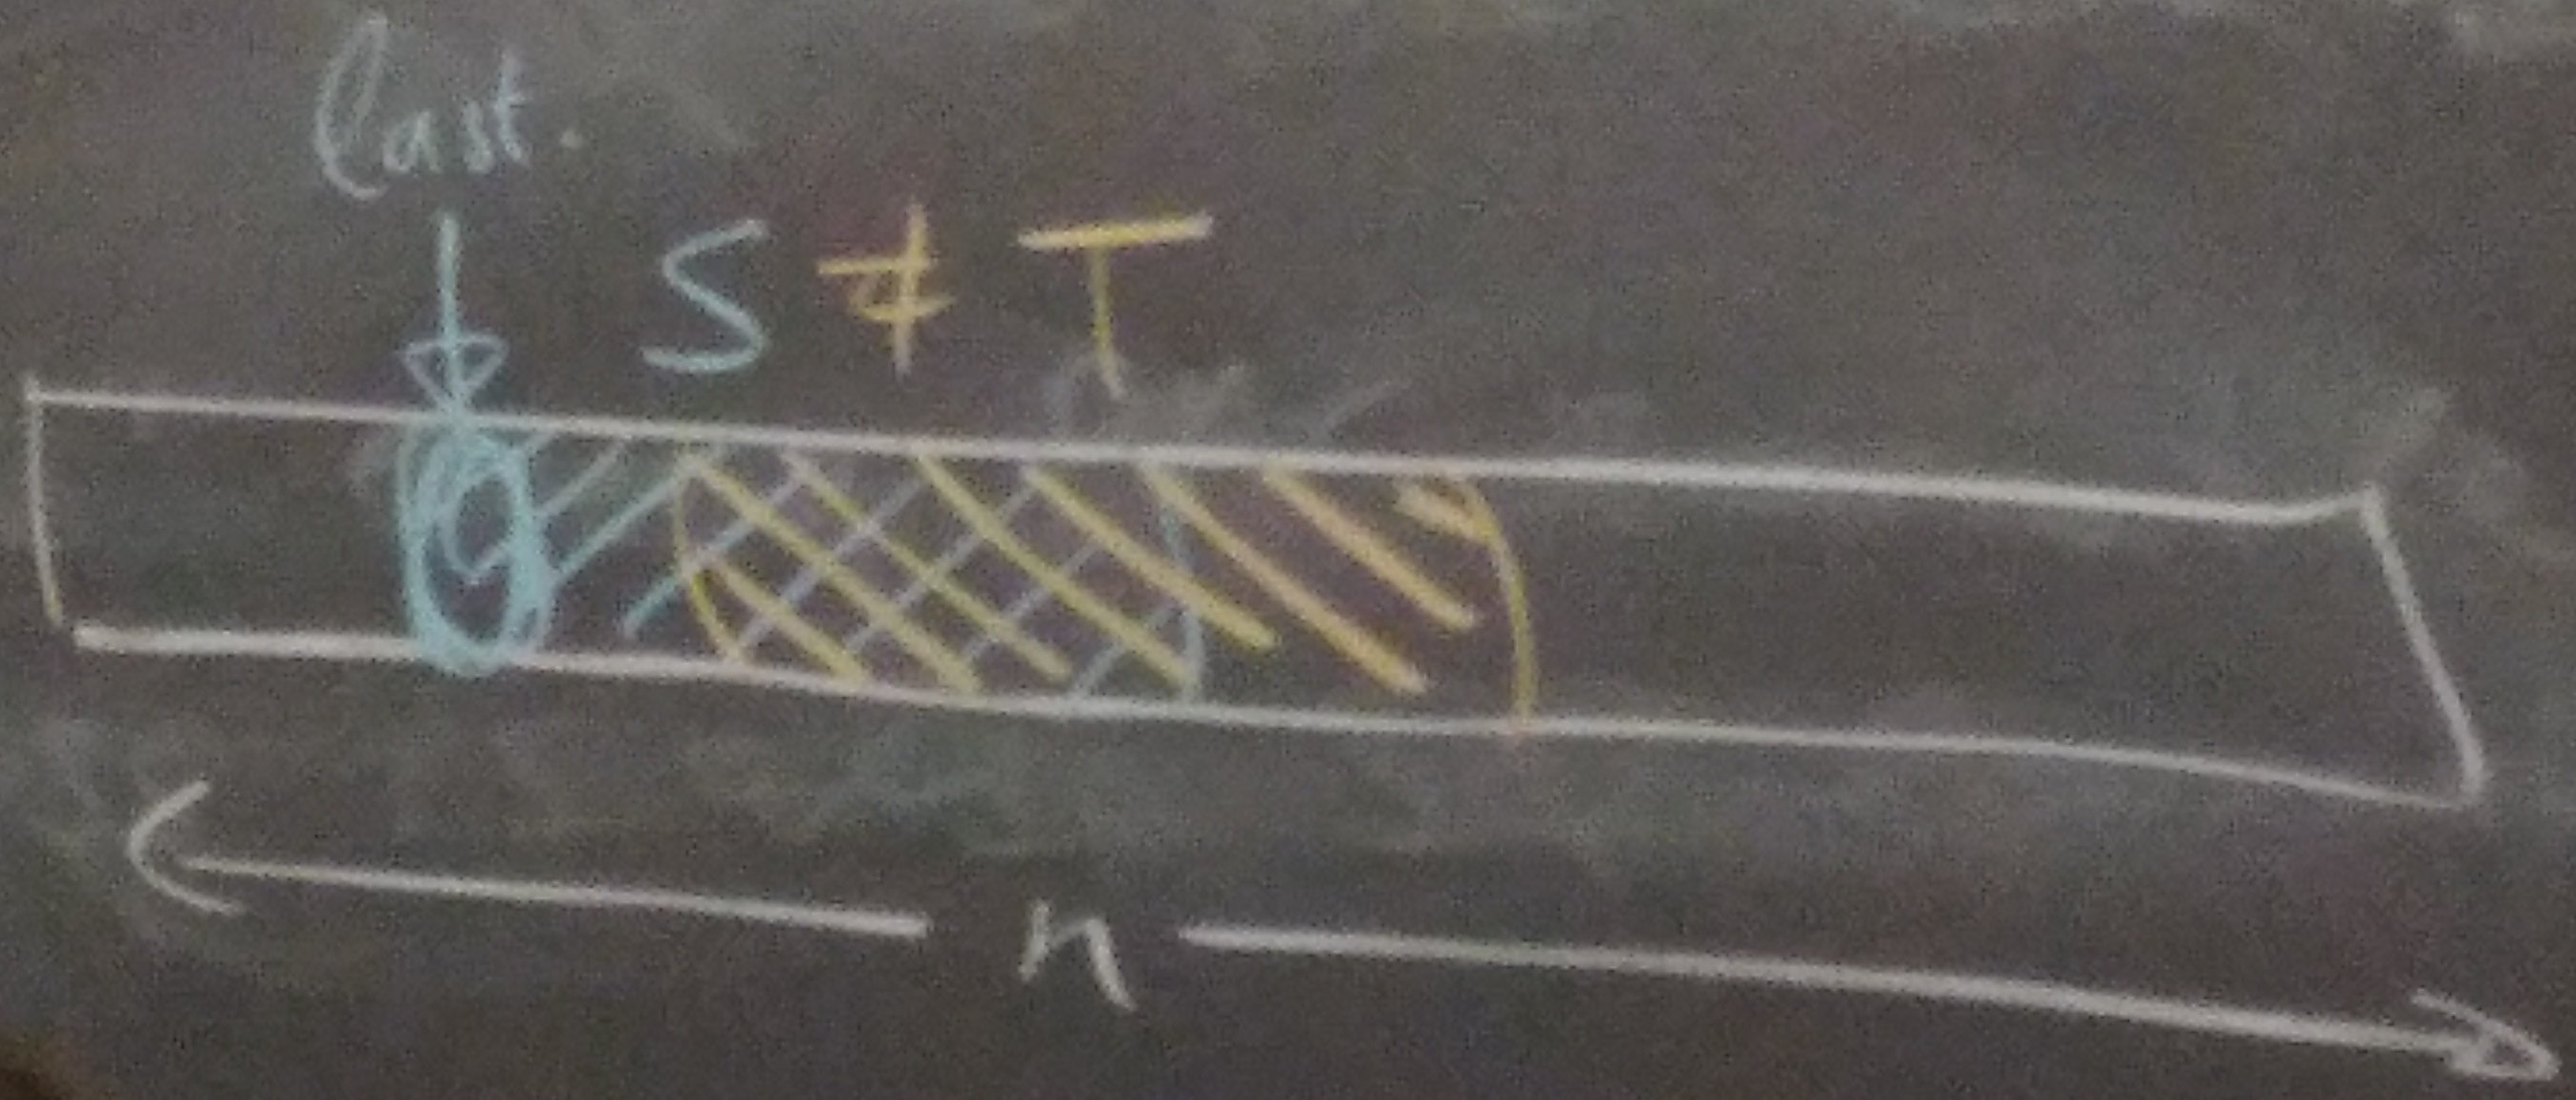
\includegraphics[width=0.6\linewidth]{img/parity.jpg}
\caption{Parity functions.}
\end{figure}
If we flip coins to decide the bits, by the time we reach the last one, T is completely determined but S relies on the result completely. 
\begin{align}
\forall S\ne T,\quad\mb P[f_S(\vec x) = f_T(\vec x)] = \frac 12 = \mb P[f_S(\vec x) \ne f_T(\vec x)]
\end{align}
Basically, the crux of the proof of ii) is proving that no matter what kind of queries we ask they reduce to the ``Is the answer this function?'' type of questions. Since, there are $2^n$ different functions we need an exponential amount of queries.
\end{proof}
We can rephrase parity functions in the following way. Take a target vector $\vec c$ in X,
\begin{align}
f_S(\vec x) = \sum_ic_ix_i \mod 2,
\end{align}
then any pair  $\langle \vec x, f_{\vec c}(\vec x)\rangle$ represents an algebraic equation on the unknowns $c_i$'s. Therefore, this can be learned in polynomial time by a PAC-learning algorithm.

\subsubsection{Characterizing Query Complexity in SQ}
\begin{definition}
We define the SQ-dimension as
\begin{multline}
SQD(\mc C, D) \coloneqq \max_d \left\{ \exists f_1,\ldots,f_d\in \mc C : \forall 1\leq i \ne j\leq d,\right.\\
\quad\quad \left.\abs{\mb P_D[f_i(x)=f_j(x)] - \mb P_D[f_i(x)\ne f_j(x)]}\leq \frac1{d^3}\right\}.
\end{multline}
Note that in the case of $\lbrace 0, 1\rbrace$, we can think of $f_i$ with labels $\pm 1$ as vectors with $2^n$ entries (corresponding to all subsets). Then, $\mb P_D[f_i(x)=f_j(x)]  - \mb P_D[f_i(x)\ne f_j(x)]$ corresponds to the inner product of $f_i$ and $f_j$. With this in mind, this definition is only saying that we want to find a large set of almost orthogonal vectors.
\end{definition}

\begin{theorem}
Let $SQ(\mc C, D)=d$, then at least $\Omega\left(d^\frac13\right)$ queries with $\tau = O\left(\frac1{d^\frac13}\right)$ are required to SQ-learn $\mc C$ wrt. D.
\end{theorem}

Recall some of the PAC-learnable classes of functions we have seen.
\begin{itemize}
\item Conjunctions over $\lbrace 0, 1\rbrace^n$
\item decisions lists (problem in the book)
\item 3-term DNF by 3CNF.
\end{itemize}
The problem is that none of the are "universal" in the sense that they cannot represent all the boolean functions. In contrast, 
\paragraph{general DNF functions:} Expressions of the form $T_1\lor\ldots\lor T_m$ where each $T_i$ is a conjunction over $x_1,\ldots,x_n,\lnot x_1,\ldots,\lnot x_n$. Now, any boolean function can be represented as a look-up table. Since we can add a $T_i$ for each of the entries of this table, they all can be represented by general DNF.

\paragraph{decision trees:}
\begin{figure}[H]
\centering
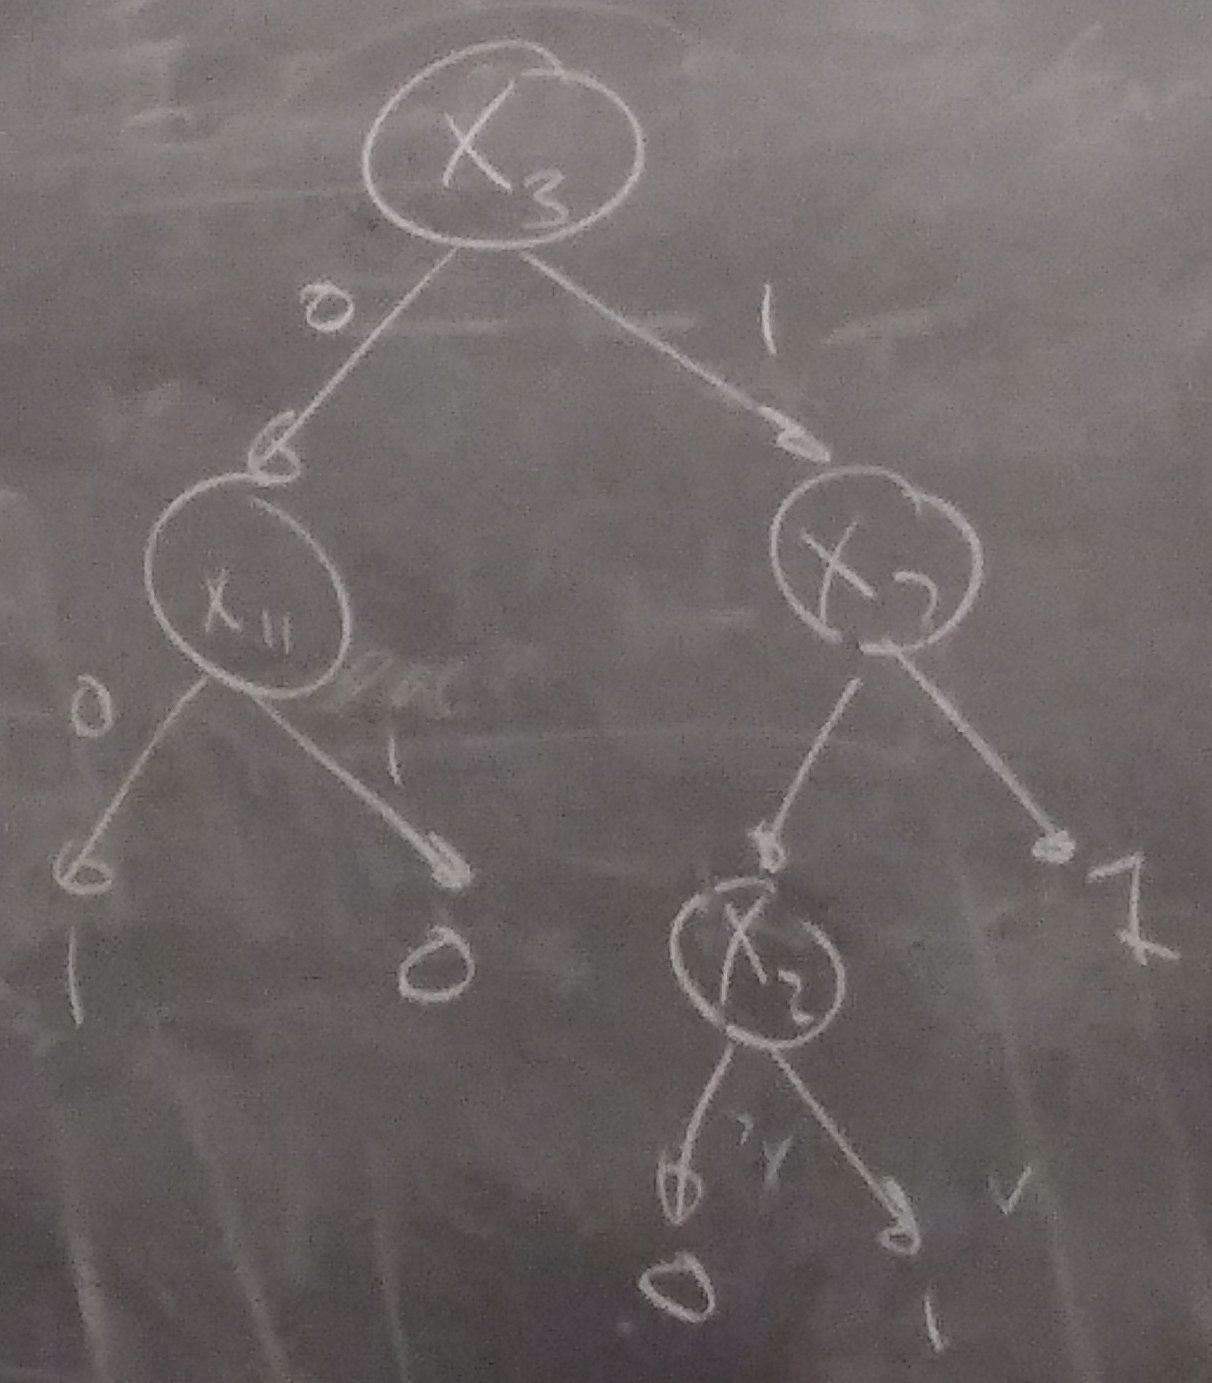
\includegraphics[width=0.6\linewidth]{img/tree}
\caption{Decision tree.}
\end{figure}
As before, we can copy the look-up table with a big enough table.

\begin{remark}
It is a big open problem whether these two classes are PAC-learnable. At least, we can use the theorem above to prove that they cannot be SQ learnable. This is in sharp contrast with the current state of the ML literature where most algorithms are SQ. This means that to PAC-learn these classes we would need radically different algorithms to the ones available at the moment.
\end{remark}

Consider parity functions $f_S(\vec x)$ where $\abs{S} = \log(n)$. We have $\binom{n}{\log (n)} \approx n^{\log(n)}$. Then, $SQD = n^{\log(n)} \rightarrow \Omega(n^{\frac{\log(n)}3})$. Consider the parity function that looks at the first $\log(n)$ bits. We can write a decision-tree to compute the parity.  This tree is a full binary tree of depth $\log(n)$.

\subsection{Learning \& Cryptography}
Recall that we saw that PAC-learning 3-term DNF by 3-term DNF is hard assuming RP $\ne$ NP. We sidestepped this by showing that 3-term DNF is PAC-learnable by 3CNF. This raises the question
\paragraph{Q:}Are there classes of functions that are hard to PAC-learn \emph{no matter} what $\mc H$ is?\\

If we allow \emph{any} hypothesis class we can always produce hypotheses that perform exhaustive search on the target class $\mc C$ until they find a consistent class with the sample. Then, everything is PAC learnable. We want to forbid these shenanigans.
\begin{figure}[H]
\centering
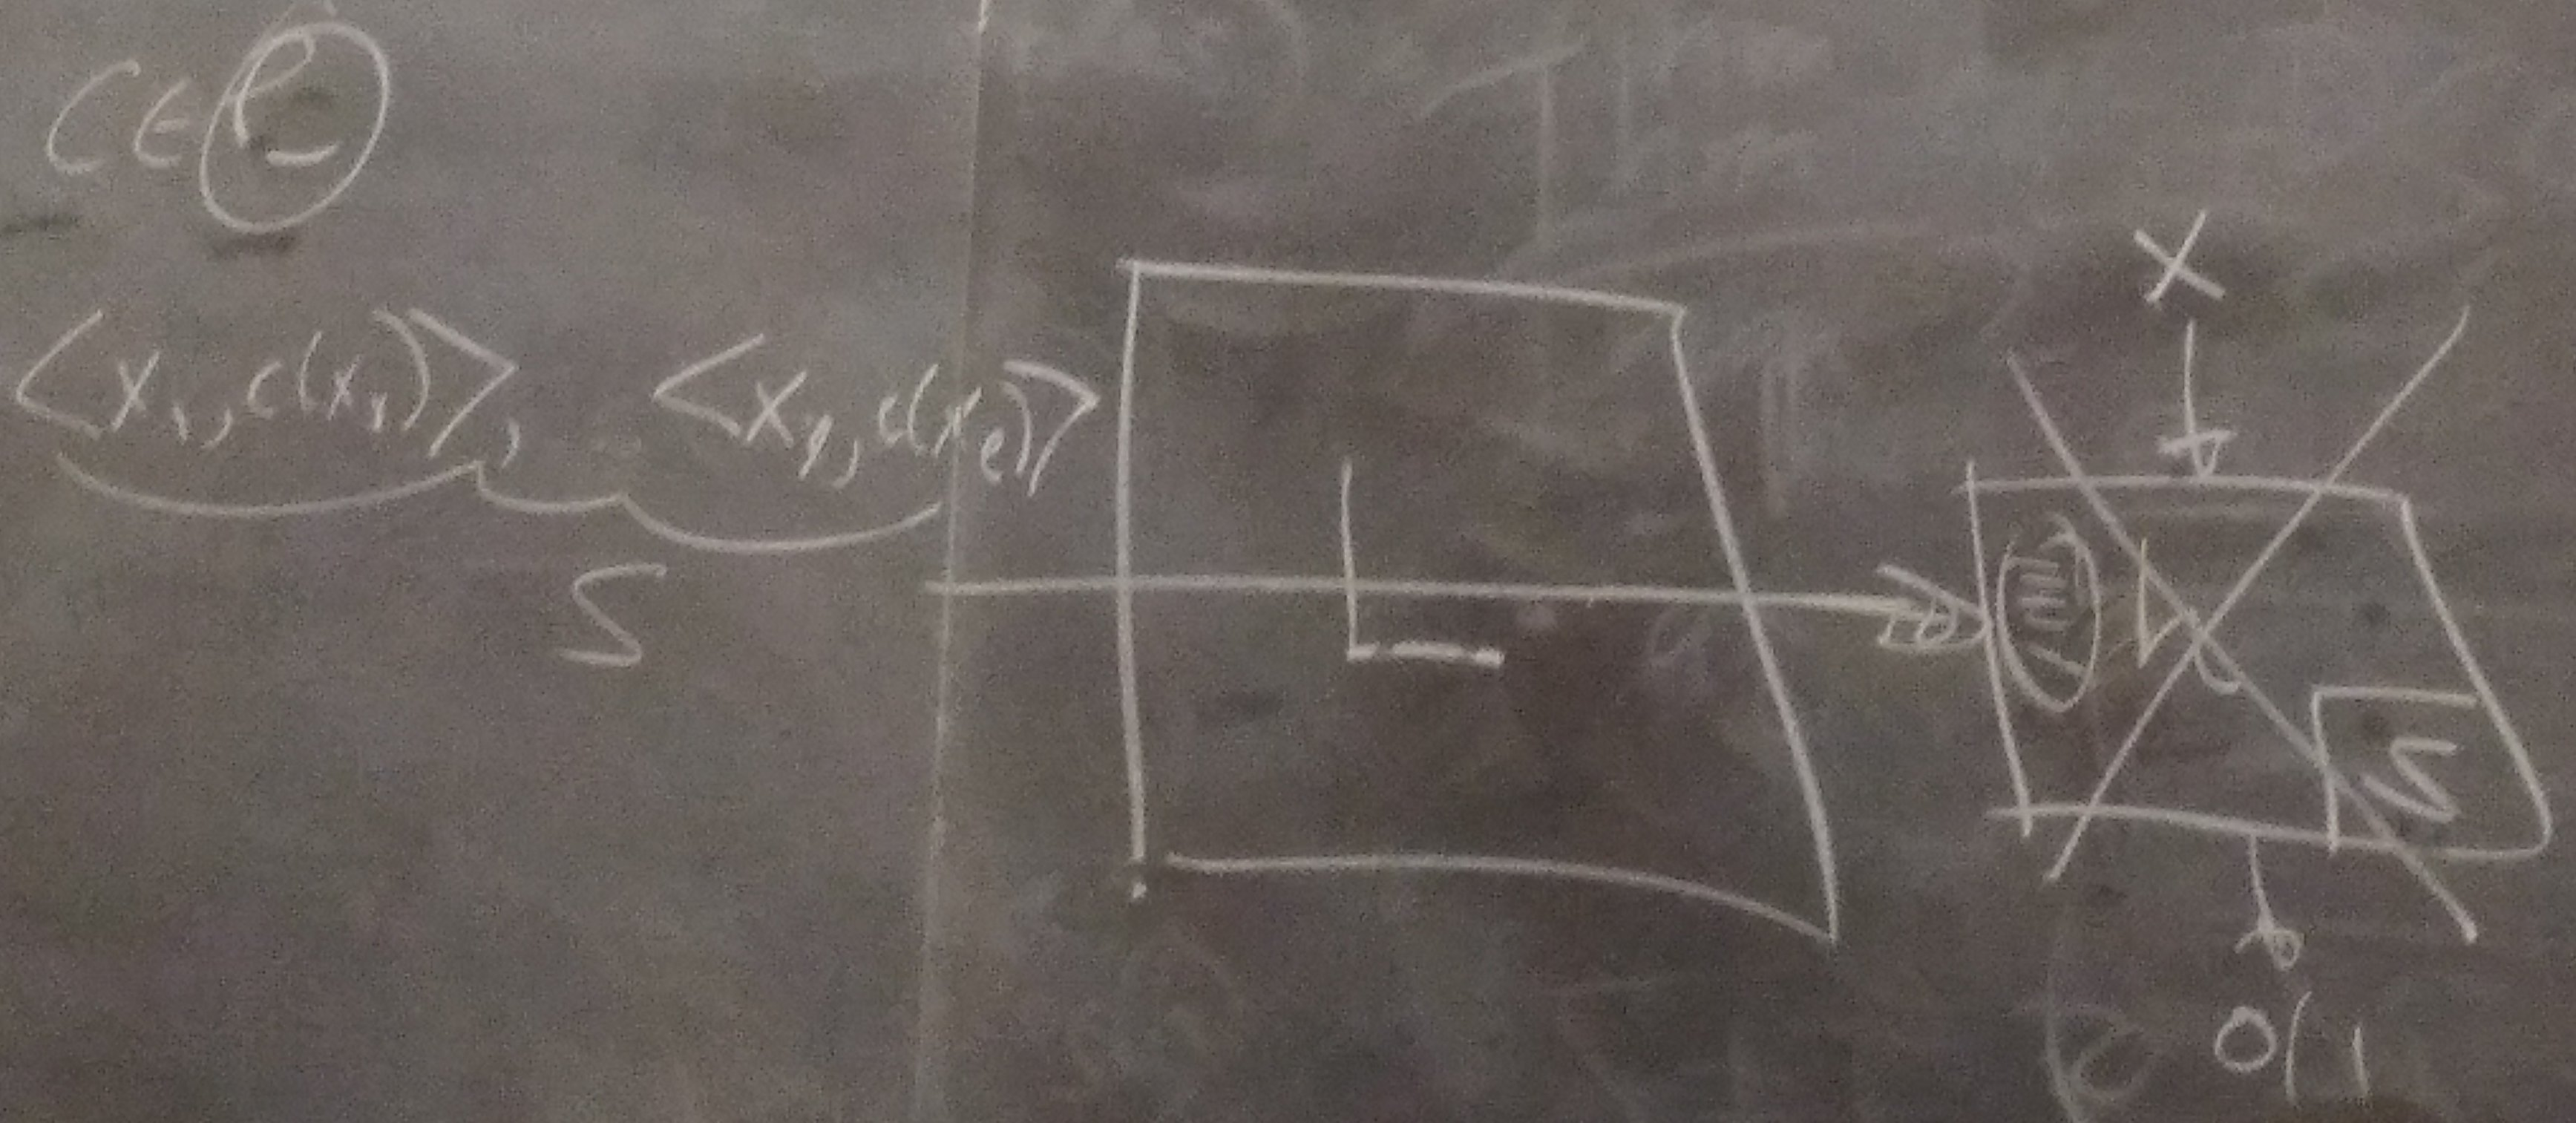
\includegraphics[width=0.6\linewidth]{img/pac.jpg}
\caption{Overpowered hypotheses.}
\end{figure}

\paragraph{Q:}Are there classes of functions that are hard to PAC-learn \emph{no matter} what \ul{polynomially evaluable} $\mc H$ we choose?

\subsubsection{Cryptography Sidebar}
\begin{itemize}
\item Alice wants to send Bob a message $\vec x\in \lbrace 0, 1\rbrace^n$ to Bob.
\item Eve is listening to the conversation between them.
\item Alice wants to encrypt her message.
\begin{figure}[H]
\centering
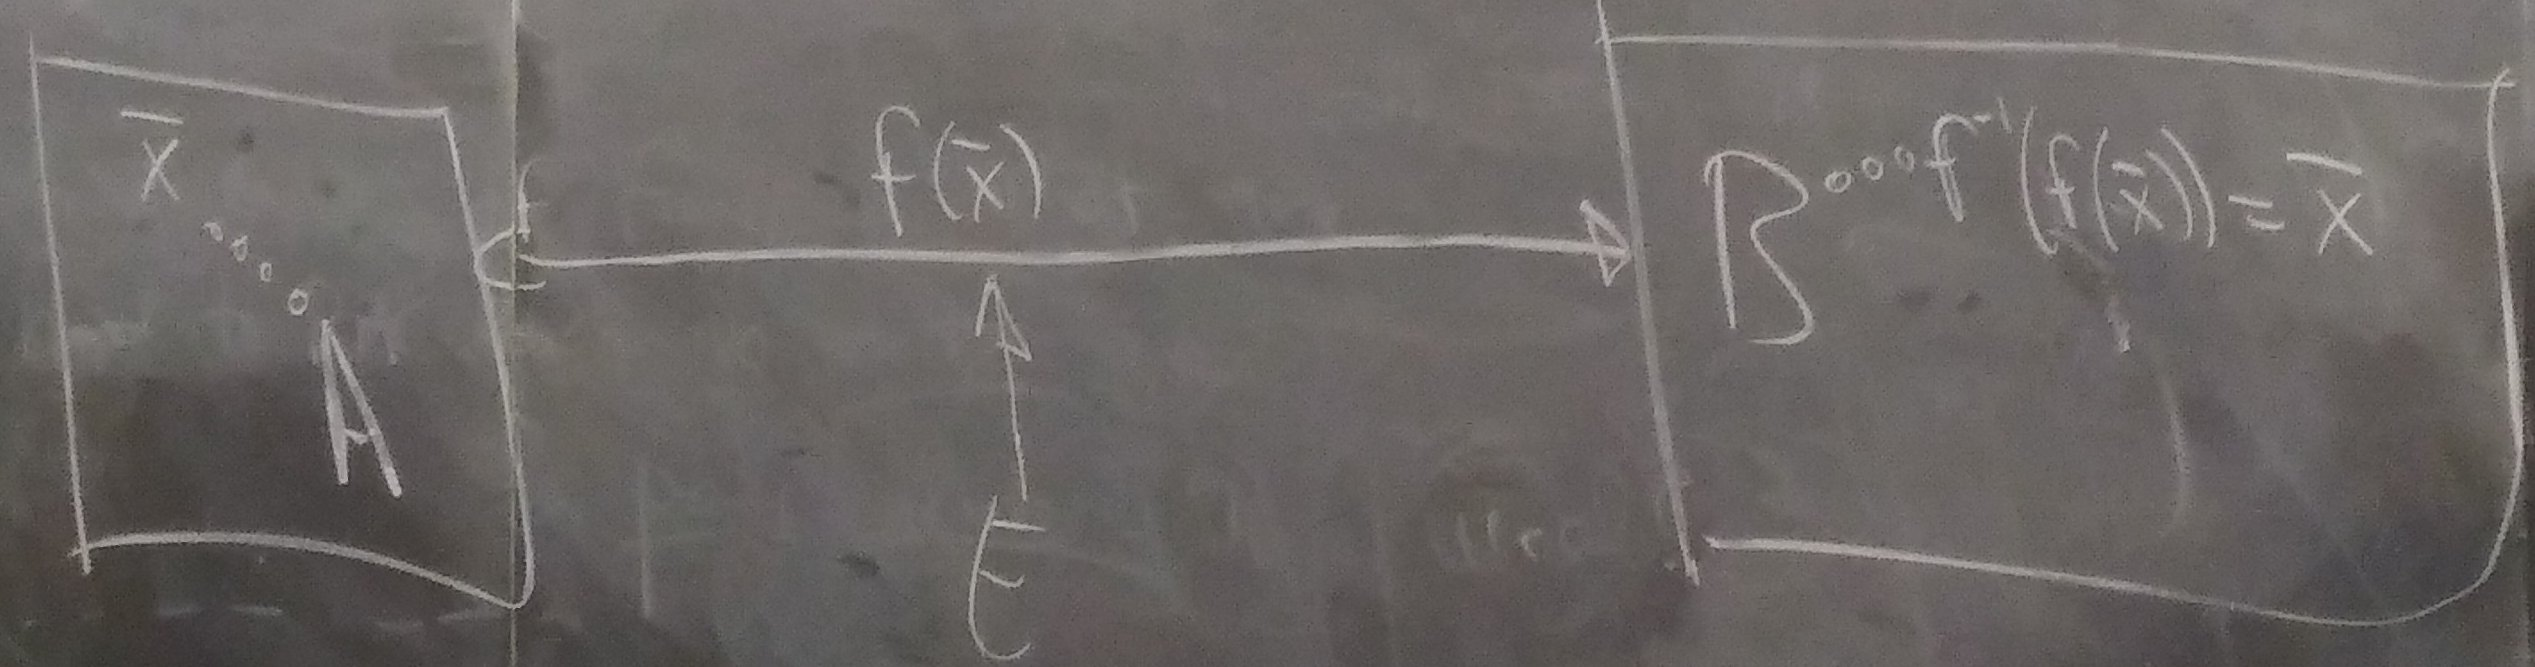
\includegraphics[width=0.6\linewidth]{img/crypto.jpg}
\caption{Cryptography layout.}
\end{figure}
\end{itemize}

\subsubsection*{One-time pad}
\begin{itemize}
\item A \& B meet privately and generate a long random bit string, $\vec z = z_1\ldots z_n$ where $z_i\in \lbrace 0,1 \rbrace$.
\item Then A sends B $f(\vec x) = \vec y$ where $y_i = x_i \oplus z_i$.
\item B can decrypt the message by doing another XOR with $\vec z$ since $(x_i \oplus z_i)\oplus z_i = x_i$
\item The message appears indistinguishable from a random one. However, it can only be used once because Eve can take XOR with previous encryptions to find out the message.
\item Not practical in the real world because you need to meet and agree on a $\vec z$ beforehand. This gives rise to public key cryptography.
\end{itemize}
Eve has a learning problem from previous deciphered messages.

\subsubsection*{Public Key Cryptography}
\begin{itemize}
\item Replace shared key/secret with \emph{two} keys for Bob:
    \begin{enumerate}
    \item \ul{public} encryption key, e
    \item \ul{private} decryption key, d
    \end{enumerate}
\item Desired data:
    \begin{enumerate}[i)]
    \item encryption $f_e(\vec x)$ is easy to compute from e
    \item $g_d(f_e(\vec x)) =\vec x$ easy to compute from d
    \item \ul{But} $g_d(\vec y)$ \emph{hard} to compute from only e, even given many encrypted/decrypted pairs (bc anybody has the public keys and can generate examples of decrypted/encrypted messages)
    \end{enumerate}
\end{itemize}

\begin{example}[RSA]
Bob chooses two random n-bit prime numbers, $p$ and $q$ and computes $N=pq$. Bob also generates a random n-bit string, e.
\begin{enumerate}
\item Bob's public key is $(N, e)$
\item To send a message x to Bob, you send $x^e\mod N$
\item From $e$, $p$ and $q$ Bob can compute a number $d$ such that $(x^e \mod N)^d \mod N = x$.
This easily satisfies $i)$ and $ii)$. Regarding $iii)$, we only need that factorizing large integers is hard.
\begin{remark}
For a slight modification of RSA, breaking it is equivalent to polynomial factorization algorithms.
\end{remark}
\end{enumerate}
\end{example}

\begin{theorem}[Not exact statement]
If factoring is hard (not in P), then the following classes are not PAC-learnable (even if we only  ask for $\ve < \frac12$):
\begin{itemize}
\item neural networks (complex enough)
\item DFA
\item boolean formuale
\end{itemize}
which are universal representations.
\end{theorem}

\end{document}
